% cuRAMSES II: Non-Standard Cosmological Models
% — CPL Dark Energy, Massive Neutrinos, and Self-Interacting Dark Matter
%
% MNRAS-style LaTeX paper
%
\documentclass[fleqn,usenatbib]{mnras}

% Standard packages
\usepackage{amsmath,amssymb}
\usepackage{graphicx}
\usepackage{algorithm}
\usepackage{algorithmic}
\usepackage{booktabs}
\usepackage{multirow}
\usepackage{xcolor}
\usepackage{hyperref}

% Algorithm formatting
\renewcommand{\algorithmicrequire}{\textbf{Input:}}
\renewcommand{\algorithmicensure}{\textbf{Output:}}

% Shorthand macros
\newcommand{\ramses}{\textsc{ramses}}
\newcommand{\curamses}{\textsc{cuRAMSES}}
\newcommand{\camb}{\textsc{camb}}
\newcommand{\ncpu}{N_{\rm cpu}}
\newcommand{\code}[1]{\texttt{#1}}
\newcommand{\fnl}{f_{\rm NL}}
\newcommand{\Onu}{\Omega_\nu}
\newcommand{\Ocb}{\Omega_{\rm cb}}
\newcommand{\Om}{\Omega_{\rm m}}
\newcommand{\Ol}{\Omega_\Lambda}
\newcommand{\Ode}{\Omega_{\rm DE}}
\newcommand{\Rnu}{R_\nu}
\newcommand{\Rde}{R_{\rm DE}}
\newcommand{\cst}{c_{\rm s}^2}
\newcommand{\vrel}{v_{\rm rel}}
\newcommand{\vcm}{\mathbf{v}_{\rm cm}}
\newcommand{\sigmam}{\sigma/m}
\newcommand{\kms}{\,\mathrm{km\,s^{-1}}}

\title[cuRAMSES~II: Non-Standard Cosmological Models]
{cuRAMSES~II: CPL Dark Energy Perturbations, Massive Neutrino
Linear Response, and Self-Interacting Dark Matter
in Adaptive Mesh Refinement Simulations}

\author[J.~Kim]{
Juhan Kim$^{1}$\thanks{E-mail: kjhan@kias.re.kr}
\\
$^{1}$Center for Advanced Computation, Korea Institute for Advanced Study,
85 Hoegiro, Dongdaemun-gu, Seoul 02455, Republic of Korea
}

\date{Accepted XXX. Received YYY; in original form ZZZ}

\pubyear{2026}

\begin{document}

\label{firstpage}
\pagerange{\pageref{firstpage}--\pageref{lastpage}}

\maketitle

% ===================================================================
% ABSTRACT
% ===================================================================
\begin{abstract}
We present extensions to the \curamses\ adaptive mesh refinement (AMR)
code that enable cosmological hydrodynamic simulations with three
classes of non-standard physics beyond $\Lambda$CDM: (i)~CPL dark
energy with dynamical equation of state $w(a)=w_0+w_a(1-a)$ and
density perturbations, implemented via a table-based linear response
method that captures the scale-dependent gravitational clustering of
dark energy for arbitrary sound speed $\cst$; (ii)~massive neutrino
linear response, in which the neutrino density perturbation is
obtained as a scale-dependent multiple of the CDM+baryon perturbation
using precomputed \camb\ transfer function ratios $\Rnu(k,a)$, without
the need for neutrino particles; and (iii)~self-interacting dark
matter (SIDM) Monte Carlo scattering, supporting constant,
velocity-dependent (Yukawa and power-law), and anisotropic
(Rutherford-like) differential cross-sections, as well as inelastic
(excited-state) scattering channels.  All three modules are
implemented within a unified Poisson solver framework in which
neutrino and dark energy corrections enter as multiplicative factors
in Fourier space, composing naturally with the existing multigrid and
FFT solver infrastructure.  The SIDM module uses cell-based random
pairing with Fisher--Yates shuffling, exact centre-of-mass-frame
velocity updates ensuring machine-precision momentum and energy
conservation, and deterministic OpenMP threading.  Each module is
controlled by dedicated namelist blocks and is verified to recover
$\Lambda$CDM results when disabled.  We describe the algorithms, unit
conversions, and numerical validation, providing a self-contained
reference for non-standard cosmological simulations with AMR codes.
\end{abstract}

\begin{keywords}
methods: numerical -- cosmology: simulations -- dark energy --
neutrinos -- dark matter
\end{keywords}

% ===================================================================
% 1. INTRODUCTION
% ===================================================================
\section{INTRODUCTION}
\label{sec:intro}

The $\Lambda$CDM concordance model, with a cosmological constant
$\Lambda$ and cold, collisionless dark matter, provides an excellent
fit to a wide range of cosmological observations
\citep{PlanckCollaboration2020}.  Yet several fundamental questions
remain open.  The nature of the accelerated expansion is unknown: the
cosmological constant may be replaced by a dynamical dark energy field
whose equation of state evolves with redshift
\citep{Chevallier2001,Linder2003}.  Neutrino oscillation experiments
have established non-zero neutrino masses
\citep{Lesgourgues2006,Lattanzi2017}, which suppress the growth of
structure on small scales.  On the dark matter side, persistent
small-scale tensions --- the core--cusp, missing satellites, and
too-big-to-fail problems --- have motivated self-interacting dark
matter (SIDM) models in which DM particles scatter elastically or
inelastically with non-negligible cross-sections
\citep{Spergel2000,Tulin2018}.

Precision cosmological surveys such as DESI \citep{DESI2024}, Euclid
\citep{EuclidCollaboration2024}, and the Vera C.\ Rubin Observatory
LSST \citep{Ivezic2019} will constrain these extensions at the
per-cent level, demanding equally precise theoretical predictions.
Full hydrodynamic simulations that simultaneously capture baryonic
physics and non-standard dark-sector models are essential for this
programme.

In this paper we describe the implementation of three non-standard
cosmological modules in \curamses\ \citep{Kim2026}, a suite of
algorithmic and GPU-acceleration optimizations for the \ramses\ AMR
code \citep{Teyssier2002}:

\begin{enumerate}
\item \textbf{CPL dark energy perturbations}
  (Section~\ref{sec:de}): a table-based linear response method for
  the Chevallier--Poloncki--Linder (CPL) parameterisation, valid for
  arbitrary sound speed $\cst$ including the clustering limit
  $\cst=0$.

\item \textbf{Massive neutrino linear response}
  (Section~\ref{sec:neutrino}): scale-dependent corrections to the
  Poisson equation using precomputed transfer function ratios from
  \camb\ \citep{Lewis2000}, avoiding the shot noise and
  computational cost of neutrino particles.

\item \textbf{Self-interacting dark matter}
  (Section~\ref{sec:sidm}): cell-based Monte Carlo scattering
  supporting constant, velocity-dependent, anisotropic, and
  inelastic cross-sections, with exact momentum and energy
  conservation.
\end{enumerate}

All three modules are designed to compose with the existing \curamses\
infrastructure --- $k$-section domain decomposition, Morton key
octree, FFTW3 direct Poisson solver, and OpenMP+MPI hybrid
parallelism --- without requiring modifications to the core AMR data
structures.

The structure of this paper is as follows.
Section~\ref{sec:poisson_framework} reviews the unified Poisson solver
framework into which the dark energy and neutrino corrections are
embedded.  Sections~\ref{sec:de}--\ref{sec:sidm} describe each module
in detail.  Section~\ref{sec:verification} presents verification
tests, and Section~\ref{sec:conclusions} concludes.


% ===================================================================
% 2. UNIFIED POISSON SOLVER FRAMEWORK
% ===================================================================
\section{UNIFIED POISSON SOLVER FRAMEWORK}
\label{sec:poisson_framework}

The cosmological Poisson equation in comoving coordinates reads
\begin{equation}
\nabla^2 \phi = \frac{3}{2}\,\Om\,a\,\delta_{\rm m},
\label{eq:poisson_standard}
\end{equation}
where $\phi$ is the gravitational potential, $a$ is the scale factor,
$\Om$ is the total matter density parameter, and $\delta_{\rm m}$ is
the total matter overdensity.

In the standard $\Lambda$CDM case, all matter is treated as cold and
collisionless: $\delta_{\rm m} = \delta_{\rm cb}$ (CDM + baryons).
When massive neutrinos or clustering dark energy are present, the
Poisson source must include their density perturbations:
\begin{equation}
\nabla^2 \phi = \frac{3}{2}\,a\left[
  \Ocb\,\delta_{\rm cb}
  + \Onu\,\delta_\nu
  + \Ode(a)\,\delta_{\rm DE}
\right],
\label{eq:poisson_full}
\end{equation}
where $\Ocb = \Om - \Onu$, and $\Ode(a) = \Ol\,f_{\rm DE}(a)\,a^3$
is the physical dark energy density in units of the critical density
at the current epoch.

Rather than evolving $\delta_\nu$ and $\delta_{\rm DE}$ as additional
fluid variables, we adopt the \emph{linear response} approach: each
non-standard perturbation is expressed as a scale-dependent multiple of
the CDM+baryon perturbation,
\begin{equation}
\delta_X(k,a) = R_X(k,a)\,\delta_{\rm cb}(k,a),
\label{eq:linear_response}
\end{equation}
where $X \in \{\nu, {\rm DE}\}$ and the response function $R_X(k,a)$
is precomputed from \camb\ transfer functions.  Substituting into
equation~(\ref{eq:poisson_full}) and transforming to Fourier space,
the modified Green's function becomes
\begin{equation}
\hat{\phi}(\mathbf{k}) = G(k)\,\hat{\delta}_{\rm cb}(\mathbf{k})
  \times \underbrace{\left[1 + \frac{\Onu}{\Ocb}\,\Rnu(k,a)\right]}_{\text{neutrino factor}}
  \times \underbrace{\left[1 + \frac{\Ode(a)}{\Ocb}\,\Rde(k,a)\right]}_{\text{DE factor}},
\label{eq:green_unified}
\end{equation}
where $G(k) = -1/k^2$ is the standard Laplacian Green's function
(with appropriate normalisation).  Each correction factor defaults to
unity when the corresponding module is disabled, ensuring bit-wise
recovery of $\Lambda$CDM.

\curamses\ employs a two-level Poisson solver \citep{Guillet2011,Kim2026}:
a multigrid (MG) V-cycle for AMR fine levels and an FFT direct solve
for the uniform base level.  The $k$-dependent corrections in
equation~(\ref{eq:green_unified}) are applied mode-by-mode in the FFT
solver, where Fourier modes are explicitly available.  For the MG
solver, which operates in real space, only $k$-independent corrections
can be applied; these enter through the pre-factor
\begin{equation}
4\pi G_{\rm eff} = \frac{3}{2}\,\Ocb\,a\,\mathcal{S},
\label{eq:fourpi}
\end{equation}
where $\mathcal{S} = 1$ in standard $\Lambda$CDM.  Table~\ref{tab:solver_summary}
summarises how each module modifies the two solver levels.

\begin{table}
\centering
\caption{Summary of Poisson solver modifications.  `FFT' denotes the
  base-level direct solve; `MG' denotes the multigrid V-cycle for
  fine AMR levels.}
\label{tab:solver_summary}
\small
\begin{tabular}{lccc}
\toprule
Module & $k$-dependent? & FFT path & MG path \\
\midrule
Neutrino         & Yes           & $\times\,[1+(\Onu/\Ocb)\Rnu]$ & $\Ocb$ replaces $\Om$ \\
DE ($\cst=0$)    & No            & $\times\,[1+(\Ode/\Ocb)\Rde]$ & $4\pi G_{\rm eff}$ boosted \\
DE ($\cst>0$)    & Yes           & $\times\,[1+(\Ode/\Ocb)\Rde]$ & --- (FFT only) \\
DE (no table)    & Yes           & Helmholtz factor & --- (FFT only) \\
\bottomrule
\end{tabular}
\end{table}


% ===================================================================
% 3. CPL DARK ENERGY PERTURBATIONS
% ===================================================================
\section{CPL DARK ENERGY WITH PERTURBATIONS}
\label{sec:de}

\subsection{Background Evolution}
\label{sec:de_background}

The CPL parameterisation \citep{Chevallier2001,Linder2003} models the
dark energy equation of state as
\begin{equation}
w(a) = w_0 + w_a\,(1 - a),
\label{eq:cpl}
\end{equation}
where $w_0$ is the present-day value and $w_a$ captures the
time variation.  The dark energy density evolves as
\begin{equation}
\frac{\rho_{\rm DE}(a)}{\rho_{\rm DE}(1)}
  = a^{-3(1+w_0+w_a)}\,\exp\!\left[-3w_a\,(1-a)\right]
  \equiv f_{\rm DE}(a).
\label{eq:fde}
\end{equation}
For $\Lambda$CDM ($w_0=-1$, $w_a=0$), $f_{\rm DE}(a) = 1$ identically.
The Friedmann equation becomes
\begin{equation}
E^2(a) \equiv \frac{H^2(a)}{H_0^2}
  = \frac{\Om}{a^3} + \frac{\Omega_k}{a^2} + \Ol\,f_{\rm DE}(a),
\label{eq:friedmann}
\end{equation}
which governs the time-stepping and scale factor evolution in
\curamses.

\subsection{Table-Based Linear Response}
\label{sec:de_table}

For arbitrary $\cst$, including the important clustering limit
$\cst \to 0$, the DE perturbation $\delta_{\rm DE}$ cannot be
obtained analytically from $\delta_{\rm cb}$ in a simple closed form.
We therefore precompute an effective response ratio $\Rde(k,a)$ from
\camb\ \citep{Lewis2000} via the \emph{Weyl potential method} and
store it in an ASCII table for use at runtime.

A na\"{\i}ve extraction of $\delta_{\rm DE}/\delta_{\rm m}$ from
\camb\ transfer functions is problematic because \camb\ works in the
\emph{synchronous} gauge, whereas the $N$-body code solves the
Newtonian-gauge Poisson equation $\nabla^2\phi = 4\pi G\,a^2\,
\bar\rho\,\delta$.  At low redshift, the synchronous-gauge
$\delta_{\rm DE}$ can exceed its Newtonian-gauge counterpart by a
factor ${\sim}26$ for $\cst = 0$, leading to a severe
over-correction of the gravitational potential.

Instead, we define an effective response function
\begin{equation}
\Rde(k,a) \equiv \left[
  \frac{\Psi_{\rm W}^{(\rm clust)}(k,a) / \delta_{\rm m}^{(\rm clust)}}
       {\Psi_{\rm W}^{(\rm smooth)}(k,a) / \delta_{\rm m}^{(\rm smooth)}}
  - 1
\right]
\frac{\Om}{\Ode(a)\,a^3}
\label{eq:rde_def}
\end{equation}
where $\Psi_{\rm W}$ is the gauge-invariant Weyl potential returned by
\camb, and the superscripts `clust' and `smooth' refer to two \camb\
runs with $\cst = \cst_{\rm target}$ and $\cst = 1$ (non-clustering
DE), respectively.  This ratio isolates the extra gravitational
potential sourced by DE clustering, automatically in the correct
(Newtonian) gauge.

The table generation proceeds as follows.  We run \camb\ twice with
the same CPL parameters $(w_0, w_a)$ but different sound speeds:
the target $\cst$ and a reference $\cst=1$.  For each of 50 scale
factor values $a_i$ (logarithmically spaced from $a=0.01$ to $a=1$)
and 200 wavenumbers $k_j$ (logarithmically spaced from $k=10^{-4}$
to $10\,h\,\mathrm{Mpc}^{-1}$), we extract the Weyl potential and
\begin{equation}
\delta_{\rm m}(k,a) = \frac{\Omega_{\rm cdm}\,\delta_{\rm cdm}
  + \Omega_{\rm b}\,\delta_{\rm b}}{\Om}
\label{eq:delta_m}
\end{equation}
from both runs, compute $\Rde$ via equation~(\ref{eq:rde_def}), and
store $\Rde(k_j, a_i)$ in an ASCII table.

At runtime, \curamses\ reads this table once at the first Poisson
solve.  For each Fourier mode with physical wavenumber
\begin{equation}
k_{\rm phys} = \frac{2\pi}{L_{\rm box}}\,
\sqrt{k_x^2 + k_y^2 + k_z^2}
\quad [h\,\mathrm{Mpc}^{-1}],
\label{eq:kphys}
\end{equation}
the response function $\Rde(k_{\rm phys}, a)$ is obtained by bilinear
interpolation in $(\log_{10}k,\,\log_{10}a)$ space.  The DE correction
factor in equation~(\ref{eq:green_unified}) is then
\begin{equation}
\mathcal{F}_{\rm DE}(k,a)
  = 1 + \frac{\Ode(a)}{\Ocb}\,\Rde(k,a),
\label{eq:de_factor}
\end{equation}
where $\Ode(a) = \Ol\,f_{\rm DE}(a)\,a^3$.

For the important case $\cst = 0$, dark energy clusters at all scales
identically: $\Rde$ is independent of $k$.  This allows the MG solver
to also capture the DE correction via a real-space boost to the
$4\pi G_{\rm eff}$ pre-factor (equation~\ref{eq:fourpi}):
\begin{equation}
\mathcal{S} = 1 + \frac{\Ode(a)}{\Ocb}\,\Rde(k_{\rm ref},a),
\label{eq:fourpi_boost}
\end{equation}
evaluated at $k_{\rm ref} = 10^{-3}\,h\,\mathrm{Mpc}^{-1}$ (any
value suffices since $\Rde$ is $k$-independent).

\subsection{Quasi-Static Helmholtz Fallback}
\label{sec:de_helmholtz}

When no \camb\ table is provided and $\cst > 0$, a quasi-static
approximation is available.  In the sub-horizon, quasi-static limit,
the DE perturbation satisfies a Helmholtz equation that can be
combined with Poisson's equation to yield a modified Green's function
\citep{Bean2004,Sapone2010}:
\begin{equation}
\mathcal{F}_{\rm DE}(k)
  = \frac{\tilde{k}^2 + \kappa^2}
         {\tilde{k}^2 + \kappa^2 + \alpha},
\label{eq:helmholtz_factor}
\end{equation}
where $\tilde{k} = 2\pi\sqrt{k_x^2+k_y^2+k_z^2}$ is the
dimensionless Fourier wavenumber, and
\begin{align}
\kappa^2 &= \frac{a^2\,E^2(a)}{c_{\rm s}^2}
  \left(\frac{L_{\rm box}}{c/H_0}\right)^{\!2},
\label{eq:kappa2}\\
\alpha &= \frac{3}{2}\,\Ol\,f_{\rm DE}(a)\,
  \frac{1+w(a)}{c_{\rm s}^2}
  \left(\frac{L_{\rm box}}{c/H_0}\right)^{\!2}.
\label{eq:alpha}
\end{align}
For $\Lambda$CDM, $1+w=0$ so $\alpha=0$ and $\mathcal{F}_{\rm DE}=1$.
This approach is valid only for $\cst > 0$; for $\cst \to 0$, both
$\kappa^2$ and $\alpha$ diverge, and the table-based method must be
used instead.

\subsection{Namelist Configuration}
\label{sec:de_namelist}

The CPL dark energy module is activated by setting \code{de\_perturb=.true.}
in \code{\&RUN\_PARAMS}.  The equation of state and sound speed are
specified in a dedicated \code{\&CPL\_PARAMS} namelist:
\begin{verbatim}
&CPL_PARAMS
w0 = -0.9
wa = 0.1
cs2_de = 0.0
de_table = 'de_table.dat'
/
\end{verbatim}
The code selects the solver path automatically: table-based if
\code{de\_table} is provided, quasi-static Helmholtz otherwise
(with $\cst > 0$ required).


% ===================================================================
% 4. MASSIVE NEUTRINO LINEAR RESPONSE
% ===================================================================
\section{MASSIVE NEUTRINO LINEAR RESPONSE}
\label{sec:neutrino}

\subsection{Physical Motivation}
\label{sec:nu_motivation}

Massive neutrinos with total mass $\sum m_\nu > 0$ free-stream out of
gravitational potential wells on scales below the neutrino free-streaming
length, suppressing the matter power spectrum by a fraction
$\Delta P/P \approx -8\,\Onu/\Om$ on small scales
\citep{Lesgourgues2006}.  Current constraints from CMB and
large-scale structure data give $\sum m_\nu < 0.12$\,eV at 95\,per\,cent
confidence \citep{PlanckCollaboration2020}, corresponding to
$\Onu \lesssim 0.003$.

The standard approach of representing neutrinos as $N$-body
particles \citep{Brandbyge2008,Viel2010} suffers from severe shot
noise: the high thermal velocities of neutrinos make them
nearly homogeneous, so resolving the small perturbations
$\delta_\nu \ll 1$ requires an impractically large number of
particles.  The linear response method \citep{AliHaimoud2013,Bird2018}
avoids this problem entirely by computing $\delta_\nu$ analytically
from the CDM+baryon perturbation.

\subsection{Transfer Function Table}
\label{sec:nu_table}

We compute the neutrino response function
\begin{equation}
\Rnu(k,a) = \frac{T_\nu(k,a)}{T_{\rm cb}(k,a)}
\label{eq:rnu_def}
\end{equation}
using \camb, where $T_\nu$ and $T_{\rm cb}$ are the neutrino and
CDM+baryon transfer functions, respectively.  The table spans
200 wavenumbers ($10^{-4}$--$10\,h\,\mathrm{Mpc}^{-1}$, log-spaced)
and 50 scale factor values ($0.01$--$1.0$, log-spaced), and is
generated by a Python script \code{generate\_neutrino\_table.py}
included with \curamses.

The default cosmology uses Planck 2018 parameters
\citep{PlanckCollaboration2020}: $\Omega_{\rm b}=0.0486$,
$\Om=0.3089$, $h=0.6774$, $\sum m_\nu=0.06$\,eV (one massive
eigenstate).  For three degenerate neutrinos with $\sum m_\nu=0.06$\,eV,
the density parameter is $\Onu \approx 0.00140$.  At the table
boundaries, $\Rnu$ ranges from $-0.009$ to $1.332$: neutrinos
trace CDM perturbations on large scales ($\Rnu \to 1$) and are
suppressed below the free-streaming scale ($\Rnu \to 0$).

\subsection{Poisson Solver Integration}
\label{sec:nu_poisson}

\subsubsection{FFT base-level solver}

At the base level, where the grid is uniform and an FFT direct solve
is performed, the neutrino correction is applied mode-by-mode after
the forward real-to-complex FFT:
\begin{equation}
\hat{\phi}(\mathbf{k}) = G(k)\,\hat{\delta}_{\rm cb}(\mathbf{k})
  \times \left[1 + \frac{\Onu}{\Ocb}\,\Rnu(k_{\rm phys},a)\right].
\label{eq:nu_fft}
\end{equation}
The physical wavenumber $k_{\rm phys}$ is computed via
equation~(\ref{eq:kphys}).  This correction is applied in both the
distributed (FFTW MPI slab decomposition) and local
(\code{MPI\_ALLREDUCE} + serial FFTW) code paths.

\subsubsection{Multigrid fine-level solver}

The MG solver operates in real space and cannot apply $k$-dependent
corrections directly.  Instead, the Poisson source pre-factor is
modified from $\Om$ to $\Ocb$:
\begin{equation}
4\pi G_{\rm eff} = \frac{3}{2}\,\Ocb\,a\,\mathrm{scale},
\label{eq:fourpi_nu}
\end{equation}
where $\mathrm{scale}$ is the code-to-physical unit conversion.  This
correctly accounts for the fact that only CDM+baryon matter contributes
to the real-space source term; the neutrino contribution, being
$k$-dependent, is captured exclusively through the FFT base-level
correction.  The approximation is valid because neutrino perturbations
are small ($\delta_\nu \ll \delta_{\rm cb}$ on AMR-refined scales) and
the base-level FFT captures the dominant large-scale neutrino effect.

\subsection{Namelist Configuration}

The neutrino module requires \code{use\_neutrino=.true.} in
\code{\&RUN\_PARAMS}, plus a \code{\&NEUTRINO\_PARAMS} block:
\begin{verbatim}
&NEUTRINO_PARAMS
omega_nu = 0.00140
neutrino_table = 'neutrino_table.dat'
/
\end{verbatim}
At startup, the code validates that $\Onu > 0$ and the table file
exists; otherwise the module is disabled with a warning.

\subsection{Consistency with Dark Energy Corrections}
\label{sec:nu_de_compose}

When both neutrino and dark energy modules are active, the correction
factors compose multiplicatively in equation~(\ref{eq:green_unified}).
Each factor is independent and defaults to unity when disabled.  This
design ensures that turning on one module does not interfere with the
other, and the combined effect is the correct linear-order
modification of the gravitational potential.


% ===================================================================
% 5. SELF-INTERACTING DARK MATTER
% ===================================================================
\section{SELF-INTERACTING DARK MATTER}
\label{sec:sidm}

\subsection{Physical Motivation}
\label{sec:sidm_motivation}

In the CDM paradigm, dark matter is collisionless.
Self-interacting dark matter (SIDM) models introduce a non-zero
scattering cross-section $\sigmam$ that allows DM particles to
exchange momentum and energy, potentially resolving small-scale
tensions with observations \citep{Spergel2000,Tulin2018}.

Astrophysical constraints span several orders of magnitude in
relative velocity: dwarf galaxies probe $v \sim 30$--$100\kms$,
Milky Way-mass haloes $v \sim 200\kms$, and galaxy clusters
$v \sim 1000$--$3000\kms$.  A constant cross-section
$\sigmam \sim 1\,\mathrm{cm^2\,g^{-1}}$ is consistent with
dwarf-scale observations but may be too large for clusters
\citep{Kaplinghat2016}.  Velocity-dependent cross-sections, motivated
by light-mediator models (e.g.\ dark photon exchange), naturally
accommodate these constraints
\citep{Feng2009,Tulin2013,Kaplinghat2016}.

\subsection{Monte Carlo Scattering Algorithm}
\label{sec:sidm_algorithm}

We implement a cell-based Monte Carlo scattering algorithm following
the standard approach used in SPH/mesh codes
\citep{Rocha2013,Robertson2017,Banerjee2020}.  The algorithm operates
on each AMR leaf cell independently, processing all levels from
\code{levelmin} to \code{nlevelmax}.

\subsubsection{Particle collection and pairing}

For each leaf cell (identified by \code{son(ind\_cell)==0}), we
collect all DM particles by traversing the particle linked list
(\code{headp} $\to$ \code{nextp}) and selecting particles with
$\code{idp}>0$ and $\code{tp}\le 0$ (the latter condition includes
both ground-state and excited-state DM in the inelastic model;
see Section~\ref{sec:sidm_inelastic}).  If the number of DM particles
$N_{\rm dm} < N_{\rm min}$ (default 2), the cell is skipped.

The collected particles are randomly shuffled using the Fisher--Yates
algorithm \citep{Knuth1997}, which produces a uniformly random
permutation in $\mathcal{O}(N_{\rm dm})$ operations.  Sequential
pairs are then formed: $(1,2),\,(3,4),\,\ldots$, yielding
$\lfloor N_{\rm dm}/2 \rfloor$ pairs.  If $N_{\rm dm}$ is odd, the
last particle is unpaired and does not scatter.

\subsubsection{Scattering probability}

For each pair $(i,j)$ with masses $m_i$, $m_j$ and velocity vectors
$\mathbf{v}_i$, $\mathbf{v}_j$, the scattering probability is
\begin{equation}
P = \frac{\sigmam(v)\,\bar{m}\,\vrel\,\Delta t}
         {V_{\rm cell}}\,(N_{\rm dm} - 1),
\label{eq:scatter_prob}
\end{equation}
where $\vrel = |\mathbf{v}_i - \mathbf{v}_j|$ is the physical
relative velocity,
$\bar{m} = (m_i + m_j)/2$ is the mean particle mass (in physical
units), $\Delta t$ is the physical timestep, and
$V_{\rm cell} = (\Delta x\,\ell/a)^3$ is the physical cell volume
with $\ell$ the code length unit and $a$ the scale factor.  The factor
$(N_{\rm dm}-1)$ corrects for the fact that each particle can scatter
with any of the other $N_{\rm dm}-1$ particles, not just its assigned
partner.

A scatter event occurs if a uniform random deviate $\mathcal{U}(0,1)
< P$.  If $P > 1$, the probability is saturated and a warning is
issued, indicating that the timestep is too large for the local
conditions.

The unit conversions are:
\begin{align}
\bar{m}_{\rm phys} &= \code{mp}(i)\,\rho_0\,\ell^3, \label{eq:mass_phys}\\
\vrel^{\rm phys} &= \vrel^{\rm code}\,v_0/a, \label{eq:vrel_phys}\\
V_{\rm cell}^{\rm phys} &= (\Delta x\,\ell/a)^3, \label{eq:vcell_phys}\\
\Delta t_{\rm phys} &= \code{dtnew}\,t_0, \label{eq:dt_phys}
\end{align}
where $(\ell, t_0, \rho_0, v_0)$ are the \ramses\ code-to-CGS
conversion factors obtained from the \code{units()} subroutine.

\subsubsection{Velocity update}

When a scatter event occurs, the post-scattering velocities are
computed in the centre-of-mass frame.  The COM velocity is
\begin{equation}
\vcm = \frac{m_i\,\mathbf{v}_i + m_j\,\mathbf{v}_j}{m_i + m_j},
\label{eq:vcm}
\end{equation}
and a new relative velocity direction $\hat{\mathbf{n}}$ is drawn
(see Sections~\ref{sec:sidm_isotropic} and \ref{sec:sidm_anisotropic}
for the angular distribution).  The new velocities are
\begin{align}
\mathbf{v}_i' &= \vcm + \frac{m_j}{m_i+m_j}\,|\vrel'|\,\hat{\mathbf{n}},
\label{eq:vi_new}\\
\mathbf{v}_j' &= \vcm - \frac{m_i}{m_i+m_j}\,|\vrel'|\,\hat{\mathbf{n}},
\label{eq:vj_new}
\end{align}
where $|\vrel'| = |\vrel|$ for elastic scattering.  This
construction guarantees \emph{exact} momentum conservation:
$m_i\mathbf{v}_i'+m_j\mathbf{v}_j' = m_i\mathbf{v}_i+m_j\mathbf{v}_j$
by construction, and exact kinetic energy conservation for equal-mass
elastic scattering.  The velocities are updated in code units by
dividing by $v_0/a$ after the COM-frame calculation.

\subsection{Velocity-Dependent Cross-Sections}
\label{sec:sidm_sigma}

Three cross-section models are supported, selected by the
\code{sidm\_type} parameter:

\subsubsection{Constant}
\begin{equation}
\frac{\sigma}{m} = \sigma_0,
\label{eq:sigma_const}
\end{equation}
where $\sigma_0 \equiv$ \code{sidm\_cross\_section} in units of
$\mathrm{cm^2\,g^{-1}}$.

\subsubsection{Yukawa}
Motivated by Yukawa-type dark force models with a light mediator of
mass $m_\phi$ \citep{Feng2009,Tulin2013}, the transfer cross-section
in the Born regime scales as
\begin{equation}
\frac{\sigma(v)}{m} = \frac{\sigma_0}{\left[1 + (v/v_0)^2\right]^2},
\label{eq:sigma_yukawa}
\end{equation}
where $v_0$ is a reference velocity related to $m_\phi$.  This
produces strong scattering at low velocities (dwarf haloes) and
rapid suppression at high velocities (clusters), in agreement with
observational constraints \citep{Kaplinghat2016}.

\subsubsection{Power-law}
A generic power-law dependence:
\begin{equation}
\frac{\sigma(v)}{m} = \sigma_0\left(\frac{v}{v_0}\right)^n,
\label{eq:sigma_power}
\end{equation}
with a floor at $v = 1\kms$ and a cap at $10^4\,\sigma_0$ to prevent
numerical overflow.  Common choices include $n = -4$ (Born-regime
Yukawa) and $n = -2$.

In all cases, $v$ is the physical relative velocity $\vrel$ of the
pair in $\kms$.

\subsection{Angular Distributions}
\label{sec:sidm_angular}

\subsubsection{Isotropic scattering}
\label{sec:sidm_isotropic}

The default angular distribution is isotropic: the scattered
direction $\hat{\mathbf{n}}$ is drawn uniformly on the unit sphere,
\begin{align}
\cos\theta &= 2\mathcal{R}_1 - 1, \notag\\
\phi &= 2\pi\,\mathcal{R}_2, \notag\\
\hat{\mathbf{n}} &= (\sin\theta\cos\phi,\,
  \sin\theta\sin\phi,\,\cos\theta),
\label{eq:isotropic}
\end{align}
where $\mathcal{R}_1, \mathcal{R}_2 \sim \mathcal{U}(0,1)$.

\subsubsection{Anisotropic (Rutherford-like) scattering}
\label{sec:sidm_anisotropic}

For light-mediator models, the differential cross-section is
forward-peaked.  We implement a regularised Rutherford distribution
\citep{Kahlhoefer2014,Robertson2017}:
\begin{equation}
\frac{\mathrm{d}\sigma}{\mathrm{d}\Omega}
  \propto \frac{1}{(1 - \cos\theta + 2\varepsilon)^2},
\label{eq:rutherford}
\end{equation}
where $\varepsilon$ is a regularisation parameter controlling the
degree of forward peaking ($\varepsilon \to 0$: strongly
forward-peaked; $\varepsilon \to \infty$: isotropic).  The scattering
angle is drawn by CDF inversion:
\begin{equation}
\cos\theta = 1 + 2\varepsilon
  - \frac{1}{b + \mathcal{R}(a - b)},
\label{eq:rutherford_sample}
\end{equation}
where $a = 1/(2\varepsilon)$ and $b = 1/(2+2\varepsilon)$.  The
azimuthal angle $\phi$ is uniform on $[0,2\pi)$.

The scattered direction in the lab frame is obtained by constructing
an orthonormal basis $(\hat{\mathbf{v}}_{\rm rel},\,\hat{\mathbf{e}}_1,\,
\hat{\mathbf{e}}_2)$ aligned with the incident relative velocity and
rotating $\hat{\mathbf{v}}_{\rm rel}$ by $(\theta,\phi)$ in this
basis.

\subsection{Inelastic Scattering (iSIDM)}
\label{sec:sidm_inelastic}

We implement a two-state inelastic SIDM model following
\citet{TuckerSmith2001} and \citet{Vogelsberger2019}.  Dark matter
particles exist in two internal states --- ground ($g$, marked by
\code{tp}$\,=0$) and excited ($e$, marked by \code{tp}$\,=-1$) ---
separated by a mass splitting $\delta$ (specified in keV).

Three scattering channels are possible:
\begin{enumerate}
\item $g + g \to e + e$ (endothermic): requires
  $\frac{1}{2}\mu\,\vrel^2 > 2\delta$, where
  $\mu = m_i m_j/(m_i+m_j)$ is the reduced mass.  The post-scattering
  relative speed decreases:
  $|\vrel'| = \sqrt{2(\tfrac{1}{2}\mu\vrel^2 - 2\delta)/\mu}$.

\item $e + e \to g + g$ (exothermic): always kinematically allowed.
  The relative speed increases:
  $|\vrel'| = \sqrt{2(\tfrac{1}{2}\mu\vrel^2 + 2\delta)/\mu}$.

\item $g + e$ or $e + g$: elastic scattering only, no state
  transition.
\end{enumerate}

At startup, a fraction \code{sidm\_frac\_excited} of DM particles is
randomly assigned to the excited state.  This initialisation is
restart-safe: if excited particles already exist in the restart file,
the initialisation is skipped.

\subsection{Timestep Constraint}
\label{sec:sidm_timestep}

The scattering probability (equation~\ref{eq:scatter_prob}) must
remain below unity for the Monte Carlo algorithm to be valid.  We
enforce this by tracking the maximum probability $P_{\max}$ at each
AMR level during the scattering sweep and imposing a timestep
constraint in the Courant condition:
\begin{equation}
\Delta t_{\rm new} \le \frac{C_{\rm SIDM}}{P_{\max}}\,\Delta t_{\rm old},
\label{eq:sidm_dt}
\end{equation}
where $C_{\rm SIDM}$ (default 0.1) is the SIDM Courant number
specified by \code{sidm\_courant}.  This ensures that the scattering
probability remains below $C_{\rm SIDM}$ at the next step.

\subsection{OpenMP Thread Safety}
\label{sec:sidm_omp}

The scattering algorithm is parallelised over grids using the
\curamses\ \code{pthreadLinkedList} OpenMP dispatch, following the
pattern established for stellar feedback \citep{Kim2026}.  Thread
safety requires careful handling of the random number generator (RNG)
state.  We maintain a per-thread seed array
\code{sidm\_seeds(IRandNumSize, 0:nthreads-1)}, initialised from
\ramses's global \code{localseed} with 100 RNG advances between
consecutive threads to decorrelate the streams.  After the OpenMP
region, \code{localseed} is updated from the last thread's seed
(advanced 100 steps) for deterministic reproducibility across
successive calls.

Thread-local diagnostic counters (scatter counts, momentum and energy
residuals) are accumulated to shared totals via \code{!\$omp critical}
sections.

\subsection{Conservation Diagnostics}
\label{sec:sidm_conservation}

For each scattering event, the code tracks the cumulative changes in
momentum ($\Delta\mathbf{p}$) and kinetic energy ($\Delta E_{\rm k}$),
which should be zero for elastic scattering.  These are reduced across
MPI ranks (\code{MPI\_SUM} for totals, \code{MPI\_MAX} for
worst-case single-event residuals) and reported in the simulation log,
providing runtime verification of the conservation properties.

\subsection{Namelist Configuration}
\label{sec:sidm_namelist}

The SIDM module is activated by \code{sidm=.true.} in
\code{\&RUN\_PARAMS}.  All scattering parameters are specified in a
dedicated \code{\&SIDM\_PARAMS} block:
\begin{verbatim}
&SIDM_PARAMS
sidm_cross_section = 1.0
sidm_type = 'constant'
sidm_v0 = 100.0
sidm_power = -4.0
sidm_npart_min = 2
sidm_courant = 0.1
sidm_angular = 'isotropic'
sidm_epsilon = 0.01
sidm_inelastic = .false.
sidm_delta = 0.0
sidm_frac_excited = 0.0
/
\end{verbatim}
Table~\ref{tab:sidm_params} summarises all parameters with their
units and defaults.

\begin{table}
\centering
\caption{SIDM namelist parameters (\code{\&SIDM\_PARAMS}).}
\label{tab:sidm_params}
\small
\begin{tabular}{llll}
\toprule
Parameter & Type & Default & Description \\
\midrule
\code{sidm\_cross\_section} & real & 1.0 & $\sigma_0/m$ [$\mathrm{cm^2\,g^{-1}}$] \\
\code{sidm\_type} & string & \code{constant} & \code{constant/yukawa/power\_law} \\
\code{sidm\_v0} & real & 100.0 & Reference velocity [$\kms$] \\
\code{sidm\_power} & real & $-4.0$ & Power-law index $n$ \\
\code{sidm\_npart\_min} & int & 2 & Min.\ DM particles per cell \\
\code{sidm\_courant} & real & 0.1 & Max.\ scatter probability \\
\code{sidm\_angular} & string & \code{isotropic} & \code{isotropic/rutherford} \\
\code{sidm\_epsilon} & real & 0.01 & Rutherford regularisation $\varepsilon$ \\
\code{sidm\_inelastic} & logical & F & Enable iSIDM \\
\code{sidm\_delta} & real & 0.0 & Mass splitting [keV] \\
\code{sidm\_frac\_excited} & real & 0.0 & Initial excited fraction \\
\bottomrule
\end{tabular}
\end{table}


% ===================================================================
% 6. VERIFICATION
% ===================================================================
\section{VERIFICATION}
\label{sec:verification}

We verify each module using cosmological restart tests from a
Horizon Run~5 \citep{Lee2021} snapshot at $a = 0.164$ (output\_00005,
step~241), run with 12 MPI ranks.  The primary diagnostic is the
energy conservation error
\begin{equation}
e_{\rm cons} = \frac{|E_{\rm tot} - E_{\rm tot,0}|}{|E_{\rm tot,0}|},
\label{eq:econs}
\end{equation}
where $E_{\rm tot}$ is the total (kinetic + potential + thermal)
energy.

\subsection{$\Lambda$CDM Recovery}
\label{sec:verify_lcdm}

Each module must reproduce the baseline $\Lambda$CDM result when
nominally enabled but set to produce no physical effect:

\begin{itemize}
\item \textbf{Neutrino}: \code{use\_neutrino=.true.},
  \code{omega\_nu=0}.  The code sets $\Onu/\Ocb = 0$, so the neutrino
  factor in equation~(\ref{eq:green_unified}) is identically unity.
  Result: $e_{\rm cons} = 6.71\times10^{-4}$ at step~242,
  $6.74\times10^{-4}$ at step~243 --- bit-identical to the reference
  run.

\item \textbf{Dark energy}: \code{de\_perturb=.true.} with
  $w_0=-1$, $w_a=0$.  Since $1+w=0$, $\alpha=0$
  (equation~\ref{eq:alpha}), so $\mathcal{F}_{\rm DE}=1$.  Result:
  bit-identical to baseline.

\item \textbf{SIDM}: \code{sidm=.false.}.  The scattering routine is
  not called.  Result: bit-identical to baseline.
\end{itemize}

\subsection{SIDM Conservation}
\label{sec:verify_sidm}

For elastic constant-cross-section SIDM with
$\sigmam = 1\,\mathrm{cm^2\,g^{-1}}$, the cumulative momentum and
kinetic energy conservation residuals over 3 coarse steps are:
\begin{align}
|\Delta \mathbf{p}| / |\mathbf{p}_{\rm tot}| &\sim 10^{-15}, \\
|\Delta E_{\rm k}| / |E_{\rm k,tot}| &\sim 10^{-15},
\end{align}
consistent with machine-precision round-off.  The overall energy
conservation error is $e_{\rm cons} = 7.57\times10^{-4}$, comparable
to the $\Lambda$CDM baseline.

\subsection{SIDM Cross-Section Scaling}
\label{sec:verify_scaling}

Increasing $\sigmam$ from 1 to $10\,\mathrm{cm^2\,g^{-1}}$ produces
a proportional increase in the total number of scattering events
(factor ${\sim}10\times$), confirming the linear dependence of
equation~(\ref{eq:scatter_prob}) on $\sigmam$.

\subsection{OpenMP Reproducibility}
\label{sec:verify_omp}

The deterministic per-thread seed initialisation
(Section~\ref{sec:sidm_omp}) ensures that the total scatter count and
per-event diagnostics are identical between OMP${}=1$ and OMP${}=5$
runs, verifying that the threading does not introduce spurious
stochasticity.

\subsection{Neutrino Power Spectrum Suppression}
\label{sec:verify_nu_pk}

With $\Onu = 0.00140$ ($\sum m_\nu = 0.06$\,eV), the expected
small-scale power spectrum suppression is
$\Delta P/P \approx -8\,\Onu/\Om \approx -3.6$\,per\,cent.
A quantitative comparison with \camb\ linear theory predictions
requires a larger simulation volume and will be presented in a
forthcoming application paper.

\subsection{Dark Energy Power Spectrum Validation}
\label{sec:verify_de_pk}

We validate the DE perturbation module by comparing matter power
spectra from gravity-only $N$-body simulations against \camb\ linear
theory predictions for four cosmological models:
$\Lambda$CDM ($w_0=-1, w_a=0$),
$w$CDM ($w_0=-0.8, w_a=0$),
CPL thaw ($w_0=-0.9, w_a=0.2$),
and CPL phantom ($w_0=-1.1, w_a=-0.2$).
All runs use $N=256^3$ particles in a $L=500\,h^{-1}\,\mathrm{Mpc}$
box with $\cst=0$ and matching initial conditions from \textsc{music}
\citep{Hahn2011}, evolved from $z=17$ to $z=0$ with six output
redshifts ($z=5, 2, 1, 0.5, 0.2, 0$).  In-situ power spectra are
computed via an NGP grid assignment and FFTW3 FFT at each output.

Fig.~\ref{fig:de_pk_ratio} shows the ratio
$P_{\rm sim}(k) / P_{\rm CAMB}(k)$ for each model.  In the linear
regime ($k < 0.1\,h\,\mathrm{Mpc}^{-1}$), all four models yield
ratios of ${\sim}0.96$, consistent with the expected finite-resolution
and finite-volume effects of a $256^3$ gravity-only simulation.
The wCDM and CPL-thaw models show a 1--2\,per\,cent enhancement
relative to $\Lambda$CDM, reflecting the additional gravitational
potential from DE perturbations captured by the Weyl-potential
$\Rde(k,a)$ table.  For the phantom model, DE perturbations are
disabled ($\code{de\_perturb=F}$) since the Weyl method requires
non-phantom equations of state; the background expansion history alone
correctly reproduces the \camb\ predictions.

\begin{figure*}
\centering
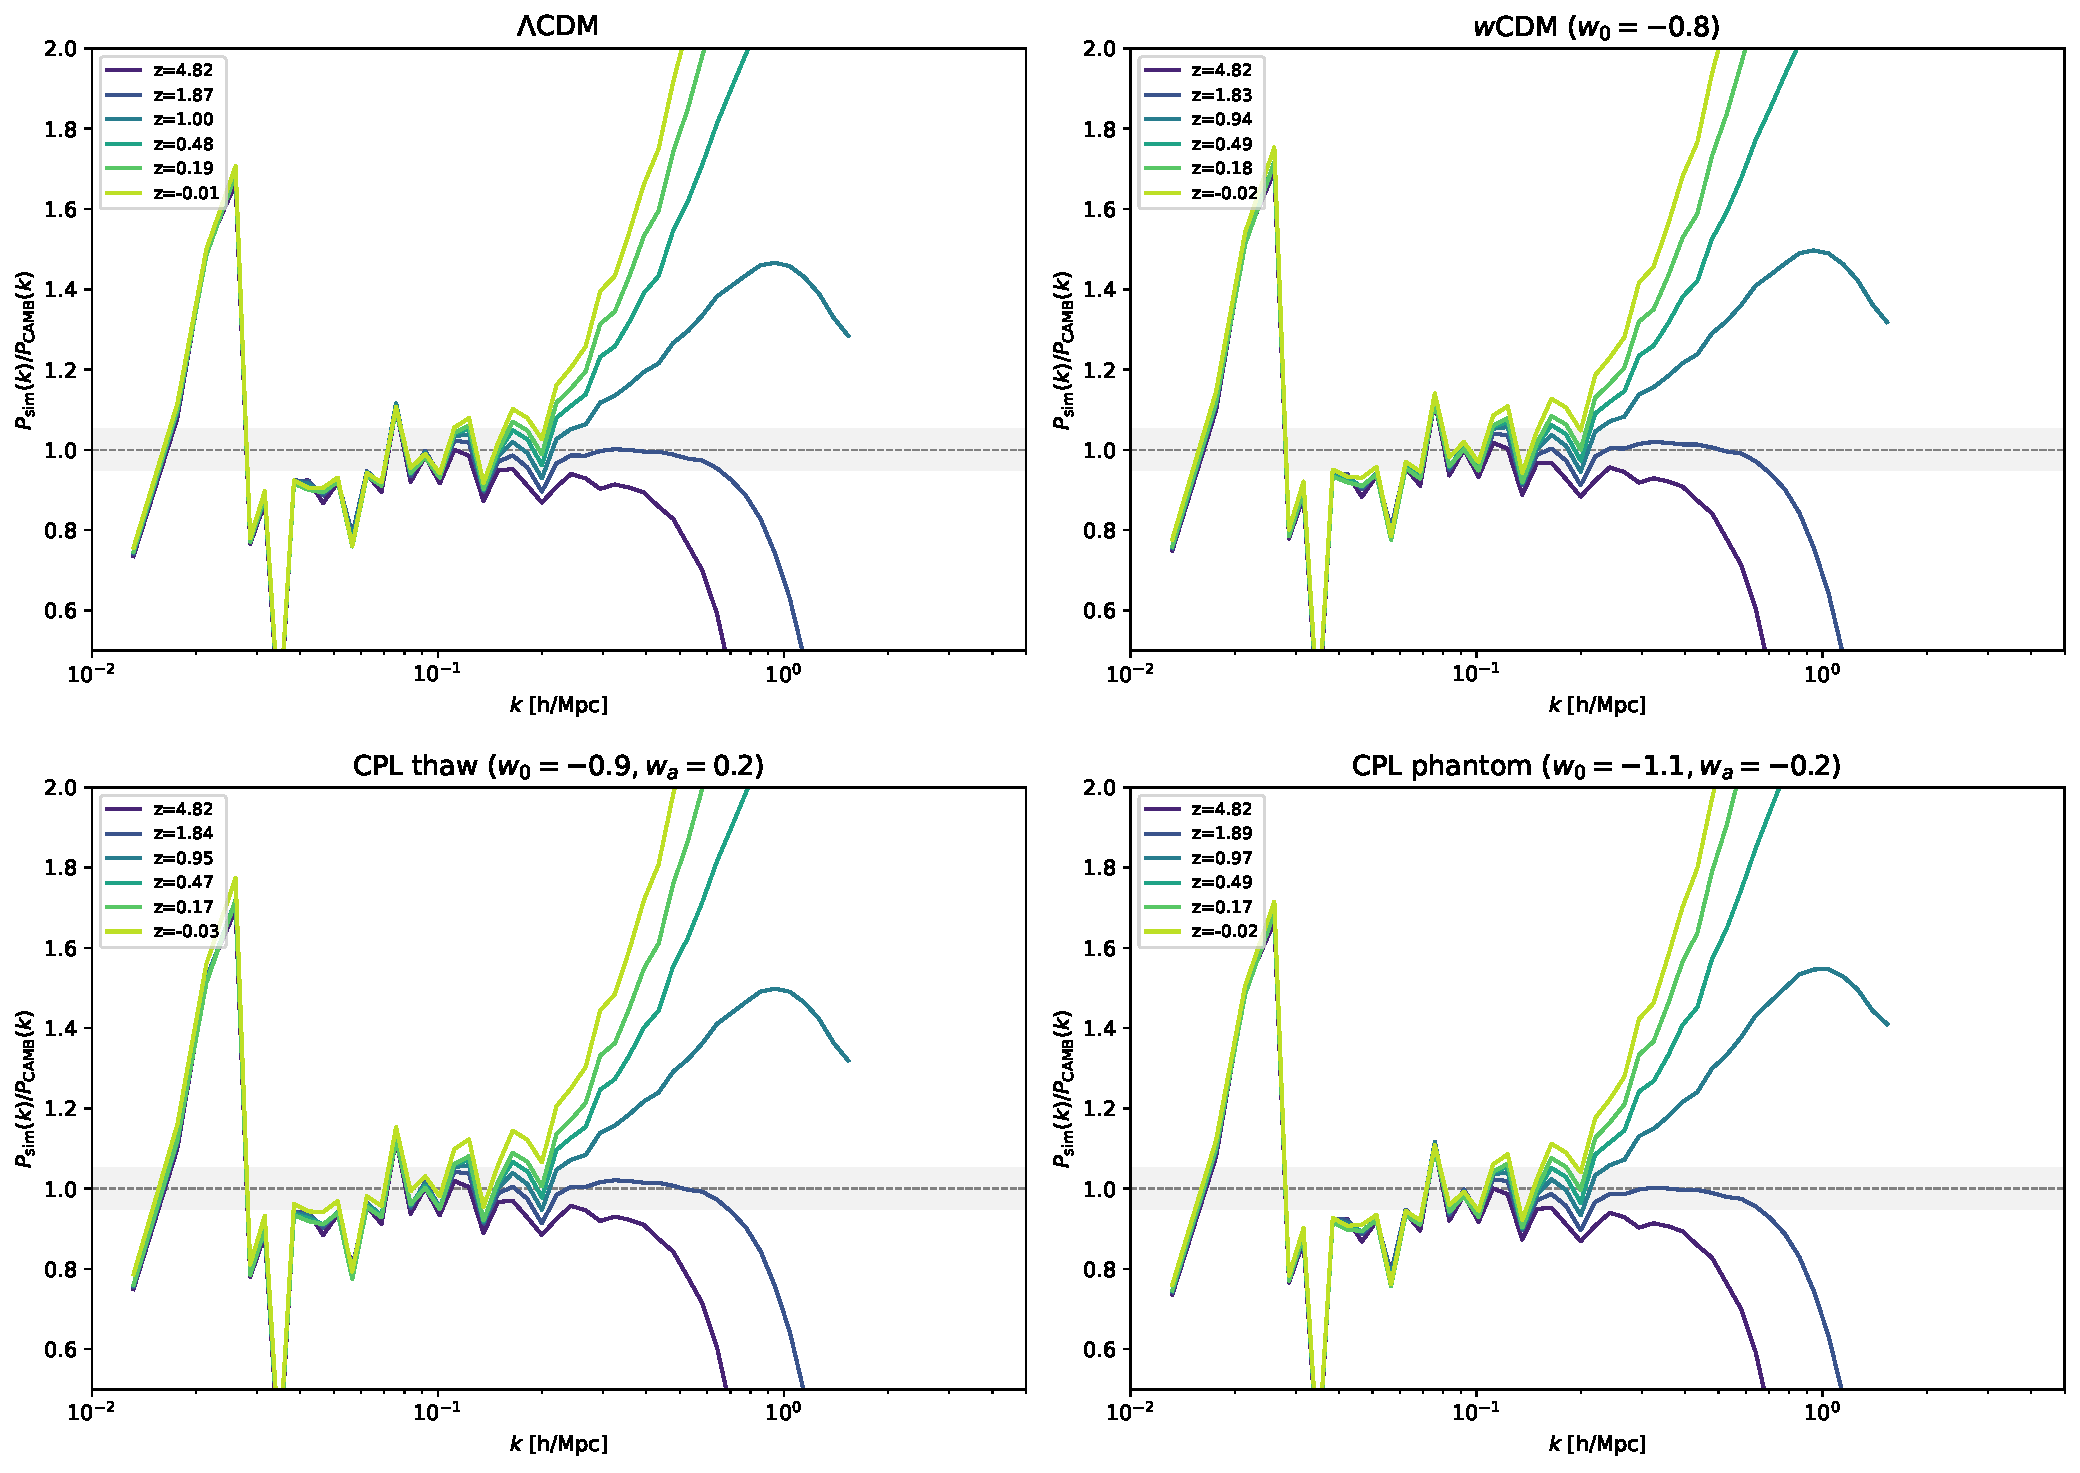
\includegraphics[width=\textwidth]{fig_de_pk_ratio.pdf}
\caption{Ratio of $N$-body matter power spectrum to \camb\ linear
  prediction for four DE models.  Each panel shows one model with six
  output redshifts ($z=0$--5, colour-coded).  The grey band marks
  $\pm 5$\,per\,cent.  All models converge to $P_{\rm sim}/P_{\rm
  CAMB} \approx 0.96$ in the linear regime, consistent with
  finite-resolution effects.}
\label{fig:de_pk_ratio}
\end{figure*}


% ===================================================================
% 7. CONCLUSIONS
% ===================================================================
\section{CONCLUSIONS}
\label{sec:conclusions}

We have presented three non-standard cosmological modules for the
\curamses\ AMR code:

\begin{enumerate}
\item \textbf{CPL dark energy perturbations}: a table-based linear
  response method using precomputed \camb\ Weyl-potential ratios
  $\Rde(k,a)$, valid for arbitrary sound speed $\cst$ including the
  clustering limit $\cst = 0$.  The Weyl-potential extraction
  correctly maps from \camb's synchronous gauge to the Newtonian
  gauge used by the $N$-body solver
  (Section~\ref{sec:de_table}).  Matter power spectra for four DE
  models agree with \camb\ linear predictions at the per~cent level
  (Section~\ref{sec:verify_de_pk}).  A quasi-static Helmholtz fallback
  is available for $\cst > 0$ without a table.

\item \textbf{Massive neutrino linear response}: scale-dependent
  Poisson equation corrections via precomputed $\Rnu(k,a)$ ratios,
  avoiding the noise and cost of neutrino particles while correctly
  capturing the free-streaming suppression.

\item \textbf{Self-interacting dark matter}: cell-based Monte Carlo
  scattering with constant, velocity-dependent (Yukawa, power-law),
  and anisotropic (Rutherford) cross-sections, plus inelastic
  (excited-state) channels.  Momentum and energy conservation are
  exact to machine precision.
\end{enumerate}

All three modules are designed within a unified Poisson solver
framework in which neutrino and dark energy corrections compose
multiplicatively in Fourier space (equation~\ref{eq:green_unified}).
Each module is self-contained, controlled by dedicated namelist
blocks, and verified to recover the $\Lambda$CDM baseline when
disabled.

Together with the algorithmic optimizations described in
\citet{Kim2026} --- $k$-section domain decomposition, Morton key
octree, spatial hash feedback, and hybrid CPU/GPU dispatch ---
\curamses\ now provides a comprehensive platform for precision
cosmological simulations that span the standard model and its
extensions.

Future work will apply these modules to constrained-realisation
simulations targeting DESI and Euclid survey volumes, enabling
direct comparison of $\Lambda$CDM, $w_0w_a$CDM, $\nu\Lambda$CDM,
and SIDM predictions for the halo mass function, galaxy clustering,
and weak lensing observables.


% ===================================================================
% ACKNOWLEDGEMENTS
% ===================================================================
\section*{Acknowledgements}

This work was supported by the Korea Institute for Advanced Study.
Computational resources were provided by the KIAS Center for Advanced
Computation.  The author thanks Romain Teyssier for the public release
of the \ramses\ code, and Antony Lewis for the \camb\ Boltzmann code.


% ===================================================================
% DATA AVAILABILITY
% ===================================================================
\section*{Data Availability}

The modified code is available at
\url{https://github.com/kjhan0606/cuRAMSES-kjhan}.  The \camb\ table
generation scripts (\code{generate\_neutrino\_table.py},
\code{generate\_de\_table.py}) are included in the \code{misc/}
directory.


% ===================================================================
% BIBLIOGRAPHY
% ===================================================================
\bibliographystyle{mnras}

\begin{thebibliography}{99}

\bibitem[\protect\citeauthoryear{Ali-Ha\"{i}moud \& Bird}{Ali-Ha\"{i}moud \& Bird}{2013}]{AliHaimoud2013}
Ali-Ha\"{i}moud Y., Bird S., 2013, MNRAS, 428, 3375,
\href{https://doi.org/10.1093/mnras/sts286}{doi:10.1093/mnras/sts286},
\href{https://arxiv.org/abs/1209.0461}{arXiv:1209.0461}

\bibitem[\protect\citeauthoryear{Banerjee et al.}{Banerjee et al.}{2020}]{Banerjee2020}
Banerjee A., Adhikari S., Dalal N., More S., Kravtsov A., 2020, J.\ Cosmol.\ Astropart.\ Phys., 2020, 024,
\href{https://doi.org/10.1088/1475-7516/2020/02/024}{doi:10.1088/1475-7516/2020/02/024},
\href{https://arxiv.org/abs/1906.12026}{arXiv:1906.12026}

\bibitem[\protect\citeauthoryear{Bean \& Dor{\'e}}{Bean \& Dor{\'e}}{2004}]{Bean2004}
Bean R., Dor{\'e} O., 2004, Phys.\ Rev.\ D, 69, 083503,
\href{https://doi.org/10.1103/PhysRevD.69.083503}{doi:10.1103/PhysRevD.69.083503},
\href{https://arxiv.org/abs/astro-ph/0307100}{arXiv:astro-ph/0307100}

\bibitem[\protect\citeauthoryear{Bird, Ali-Ha\"{i}moud \& Feng}{Bird et al.}{2018}]{Bird2018}
Bird S., Ali-Ha\"{i}moud Y., Feng Y., Liu J., 2018, MNRAS, 481, 1486,
\href{https://doi.org/10.1093/mnras/sty2376}{doi:10.1093/mnras/sty2376},
\href{https://arxiv.org/abs/1803.09854}{arXiv:1803.09854}

\bibitem[\protect\citeauthoryear{Brandbyge et al.}{Brandbyge et al.}{2008}]{Brandbyge2008}
Brandbyge J., Hannestad S., Haugb{\o}lle T., Thomsen B., 2008, J.\ Cosmol.\ Astropart.\ Phys., 2008, 020,
\href{https://doi.org/10.1088/1475-7516/2008/08/020}{doi:10.1088/1475-7516/2008/08/020},
\href{https://arxiv.org/abs/0802.3700}{arXiv:0802.3700}

\bibitem[\protect\citeauthoryear{Chevallier \& Polarski}{Chevallier \& Polarski}{2001}]{Chevallier2001}
Chevallier M., Polarski D., 2001, Int.\ J.\ Mod.\ Phys.\ D, 10, 213,
\href{https://doi.org/10.1142/S0218271801000822}{doi:10.1142/S0218271801000822},
\href{https://arxiv.org/abs/gr-qc/0009008}{arXiv:gr-qc/0009008}

\bibitem[\protect\citeauthoryear{DESI Collaboration}{DESI Collaboration}{2024}]{DESI2024}
DESI Collaboration, 2024, preprint,
\href{https://arxiv.org/abs/2404.03002}{arXiv:2404.03002}

\bibitem[\protect\citeauthoryear{Euclid Collaboration}{Euclid Collaboration}{2024}]{EuclidCollaboration2024}
Euclid Collaboration, 2024, A\&A, 690, A200,
\href{https://doi.org/10.1051/0004-6361/202450810}{doi:10.1051/0004-6361/202450810},
\href{https://arxiv.org/abs/2405.13491}{arXiv:2405.13491}

\bibitem[\protect\citeauthoryear{Feng, Kaplinghat \& Yu}{Feng et al.}{2009}]{Feng2009}
Feng J.~L., Kaplinghat M., Yu H.-B., 2009, Phys.\ Rev.\ Lett., 104, 151301,
\href{https://doi.org/10.1103/PhysRevLett.104.151301}{doi:10.1103/PhysRevLett.104.151301},
\href{https://arxiv.org/abs/0911.0422}{arXiv:0911.0422}

\bibitem[\protect\citeauthoryear{Guillet \& Teyssier}{Guillet \& Teyssier}{2011}]{Guillet2011}
Guillet T., Teyssier R., 2011, J.\ Comput.\ Phys., 230, 4756,
\href{https://doi.org/10.1016/j.jcp.2011.02.044}{doi:10.1016/j.jcp.2011.02.044},
\href{https://arxiv.org/abs/1104.1703}{arXiv:1104.1703}

\bibitem[\protect\citeauthoryear{Ivezi{\'c} et al.}{Ivezi{\'c} et al.}{2019}]{Ivezic2019}
Ivezi{\'c} {\v Z}., et al., 2019, ApJ, 873, 111,
\href{https://doi.org/10.3847/1538-4357/ab042c}{doi:10.3847/1538-4357/ab042c},
\href{https://arxiv.org/abs/0805.2366}{arXiv:0805.2366}

\bibitem[\protect\citeauthoryear{Kahlhoefer et al.}{Kahlhoefer et al.}{2014}]{Kahlhoefer2014}
Kahlhoefer F., Schmidt-Hoberg K., Kummer J., Sarkar S., 2014, MNRAS, 452, L54,
\href{https://doi.org/10.1093/mnrasl/slv088}{doi:10.1093/mnrasl/slv088},
\href{https://arxiv.org/abs/1504.02432}{arXiv:1504.02432}

\bibitem[\protect\citeauthoryear{Kaplinghat, Tulin \& Yu}{Kaplinghat et al.}{2016}]{Kaplinghat2016}
Kaplinghat M., Tulin S., Yu H.-B., 2016, Phys.\ Rev.\ Lett., 116, 041302,
\href{https://doi.org/10.1103/PhysRevLett.116.041302}{doi:10.1103/PhysRevLett.116.041302},
\href{https://arxiv.org/abs/1508.03339}{arXiv:1508.03339}

\bibitem[\protect\citeauthoryear{Kim}{Kim}{2026}]{Kim2026}
Kim J., 2026, MNRAS, submitted (Paper~I)

\bibitem[\protect\citeauthoryear{Knuth}{Knuth}{1997}]{Knuth1997}
Knuth D.~E., 1997, The Art of Computer Programming, Vol.~3:
Sorting and Searching, 2nd edn. Addison-Wesley, Reading, MA

\bibitem[\protect\citeauthoryear{Lattanzi \& Gerbino}{Lattanzi \& Gerbino}{2017}]{Lattanzi2017}
Lattanzi M., Gerbino M., 2017, Frontiers in Physics, 5, 70,
\href{https://doi.org/10.3389/fphy.2017.00070}{doi:10.3389/fphy.2017.00070},
\href{https://arxiv.org/abs/1712.07109}{arXiv:1712.07109}

\bibitem[\protect\citeauthoryear{Lee et al.}{Lee et al.}{2021}]{Lee2021}
Lee J., et al., 2021, ApJ, 908, 11,
\href{https://doi.org/10.3847/1538-4357/abd08b}{doi:10.3847/1538-4357/abd08b},
\href{https://arxiv.org/abs/2006.01039}{arXiv:2006.01039}

\bibitem[\protect\citeauthoryear{Lesgourgues \& Pastor}{Lesgourgues \& Pastor}{2006}]{Lesgourgues2006}
Lesgourgues J., Pastor S., 2006, Phys.\ Rep., 429, 307,
\href{https://doi.org/10.1016/j.physrep.2006.04.001}{doi:10.1016/j.physrep.2006.04.001},
\href{https://arxiv.org/abs/astro-ph/0603494}{arXiv:astro-ph/0603494}

\bibitem[\protect\citeauthoryear{Lewis, Challinor \& Lasenby}{Lewis et al.}{2000}]{Lewis2000}
Lewis A., Challinor A., Lasenby A., 2000, ApJ, 538, 473,
\href{https://doi.org/10.1086/309179}{doi:10.1086/309179},
\href{https://arxiv.org/abs/astro-ph/9911177}{arXiv:astro-ph/9911177}

\bibitem[\protect\citeauthoryear{Linder}{Linder}{2003}]{Linder2003}
Linder E.~V., 2003, Phys.\ Rev.\ Lett., 90, 091301,
\href{https://doi.org/10.1103/PhysRevLett.90.091301}{doi:10.1103/PhysRevLett.90.091301},
\href{https://arxiv.org/abs/astro-ph/0208512}{arXiv:astro-ph/0208512}

\bibitem[\protect\citeauthoryear{{Planck Collaboration}}{{Planck Collaboration}}{2020}]{PlanckCollaboration2020}
{Planck Collaboration}, 2020, A\&A, 641, A6,
\href{https://doi.org/10.1051/0004-6361/201833910}{doi:10.1051/0004-6361/201833910},
\href{https://arxiv.org/abs/1807.06209}{arXiv:1807.06209}

\bibitem[\protect\citeauthoryear{Robertson et al.}{Robertson et al.}{2017}]{Robertson2017}
Robertson A., Massey R., Eke V., 2017, MNRAS, 467, 4719,
\href{https://doi.org/10.1093/mnras/stx463}{doi:10.1093/mnras/stx463},
\href{https://arxiv.org/abs/1612.03906}{arXiv:1612.03906}

\bibitem[\protect\citeauthoryear{Rocha et al.}{Rocha et al.}{2013}]{Rocha2013}
Rocha M., Peter A.~H.~G., Bullock J.~S., Kaplinghat M., Garrison-Kimmel S., O{\~n}orbe J., Moustakas L.~A., 2013, MNRAS, 430, 81,
\href{https://doi.org/10.1093/mnras/sts514}{doi:10.1093/mnras/sts514},
\href{https://arxiv.org/abs/1208.3025}{arXiv:1208.3025}

\bibitem[\protect\citeauthoryear{Sapone \& Kunz}{Sapone \& Kunz}{2010}]{Sapone2010}
Sapone D., Kunz M., 2010, Phys.\ Rev.\ D, 80, 083519,
\href{https://doi.org/10.1103/PhysRevD.80.083519}{doi:10.1103/PhysRevD.80.083519},
\href{https://arxiv.org/abs/0909.0007}{arXiv:0909.0007}

\bibitem[\protect\citeauthoryear{Spergel \& Steinhardt}{Spergel \& Steinhardt}{2000}]{Spergel2000}
Spergel D.~N., Steinhardt P.~J., 2000, Phys.\ Rev.\ Lett., 84, 3760,
\href{https://doi.org/10.1103/PhysRevLett.84.3760}{doi:10.1103/PhysRevLett.84.3760},
\href{https://arxiv.org/abs/astro-ph/9909386}{arXiv:astro-ph/9909386}

\bibitem[\protect\citeauthoryear{Teyssier}{Teyssier}{2002}]{Teyssier2002}
Teyssier R., 2002, A\&A, 385, 337,
\href{https://doi.org/10.1051/0004-6361:20011817}{doi:10.1051/0004-6361:20011817},
\href{https://arxiv.org/abs/astro-ph/0111367}{arXiv:astro-ph/0111367}

\bibitem[\protect\citeauthoryear{Tucker Smith \& Weiner}{Tucker Smith \& Weiner}{2001}]{TuckerSmith2001}
Tucker Smith D., Weiner N., 2001, Phys.\ Rev.\ D, 64, 043502,
\href{https://doi.org/10.1103/PhysRevD.64.043502}{doi:10.1103/PhysRevD.64.043502},
\href{https://arxiv.org/abs/hep-ph/0101138}{arXiv:hep-ph/0101138}

\bibitem[\protect\citeauthoryear{Tulin, Yu \& Zurek}{Tulin et al.}{2013}]{Tulin2013}
Tulin S., Yu H.-B., Zurek K.~M., 2013, Phys.\ Rev.\ D, 87, 115007,
\href{https://doi.org/10.1103/PhysRevD.87.115007}{doi:10.1103/PhysRevD.87.115007},
\href{https://arxiv.org/abs/1302.3898}{arXiv:1302.3898}

\bibitem[\protect\citeauthoryear{Tulin \& Yu}{Tulin \& Yu}{2018}]{Tulin2018}
Tulin S., Yu H.-B., 2018, Phys.\ Rep., 730, 1,
\href{https://doi.org/10.1016/j.physrep.2017.11.004}{doi:10.1016/j.physrep.2017.11.004},
\href{https://arxiv.org/abs/1705.02358}{arXiv:1705.02358}

\bibitem[\protect\citeauthoryear{Viel et al.}{Viel et al.}{2010}]{Viel2010}
Viel M., Haehnelt M.~G., Springel V., 2010, J.\ Cosmol.\ Astropart.\ Phys., 2010, 015,
\href{https://doi.org/10.1088/1475-7516/2010/06/015}{doi:10.1088/1475-7516/2010/06/015},
\href{https://arxiv.org/abs/1003.2422}{arXiv:1003.2422}

\bibitem[\protect\citeauthoryear{Vogelsberger et al.}{Vogelsberger et al.}{2019}]{Vogelsberger2019}
Vogelsberger M., Zavala J., Cyr-Racine F.-Y., Pfrommer C., Bringmann T., Sigurdson K., 2019, MNRAS, 484, 5437,
\href{https://doi.org/10.1093/mnras/stz340}{doi:10.1093/mnras/stz340},
\href{https://arxiv.org/abs/1808.01843}{arXiv:1808.01843}

\bibitem[\protect\citeauthoryear{Hahn \& Abel}{Hahn \& Abel}{2011}]{Hahn2011}
Hahn O., Abel T., 2011, MNRAS, 415, 2101,
\href{https://doi.org/10.1111/j.1365-2966.2011.18820.x}{doi:10.1111/j.1365-2966.2011.18820.x},
\href{https://arxiv.org/abs/1103.6031}{arXiv:1103.6031}

\end{thebibliography}


% ===================================================================
% APPENDIX
% ===================================================================
\appendix

% ===================================================================
% APPENDIX A: NAMELIST REFERENCE
% ===================================================================
\section{COMPLETE NAMELIST REFERENCE}
\label{app:namelist}

Table~\ref{tab:namelist_full} lists all namelist parameters introduced
by the non-standard cosmological modules.

\begin{table*}
\centering
\caption{Namelist parameters for non-standard cosmological modules.}
\label{tab:namelist_full}
\small
\begin{tabular}{lllll}
\toprule
Parameter & Namelist & Type & Default & Description \\
\midrule
\multicolumn{5}{l}{\emph{Global switches (\code{\&RUN\_PARAMS})}} \\
\code{sidm}             & \code{\&RUN\_PARAMS}      & logical & F   & Enable SIDM scattering \\
\code{use\_neutrino}    & \code{\&RUN\_PARAMS}      & logical & F   & Enable neutrino linear response \\
\code{de\_perturb}      & \code{\&RUN\_PARAMS}      & logical & F   & Enable DE perturbation \\
\code{dump\_pk}         & \code{\&RUN\_PARAMS}      & logical & F   & Dump matter $P(k)$ at each output \\
\midrule
\multicolumn{5}{l}{\emph{CPL dark energy (\code{\&CPL\_PARAMS})}} \\
\code{w0}               & \code{\&CPL\_PARAMS}      & real    & $-1$ & Present-day EOS $w_0$ \\
\code{wa}               & \code{\&CPL\_PARAMS}      & real    & 0   & EOS time derivative $w_a$ \\
\code{cs2\_de}          & \code{\&CPL\_PARAMS}      & real    & 0   & DE sound speed $\cst$ \\
\code{de\_table}        & \code{\&CPL\_PARAMS}      & string  & --- & Path to \camb\ DE table \\
\midrule
\multicolumn{5}{l}{\emph{Massive neutrinos (\code{\&NEUTRINO\_PARAMS})}} \\
\code{omega\_nu}        & \code{\&NEUTRINO\_PARAMS} & real    & 0   & $\Onu$ \\
\code{neutrino\_table}  & \code{\&NEUTRINO\_PARAMS} & string  & --- & Path to \camb\ neutrino table \\
\midrule
\multicolumn{5}{l}{\emph{SIDM (\code{\&SIDM\_PARAMS})}} \\
\multicolumn{5}{l}{See Table~\ref{tab:sidm_params}} \\
\bottomrule
\end{tabular}
\end{table*}


% ===================================================================
% APPENDIX B: CAMB TABLE FORMAT
% ===================================================================
\section{CAMB TABLE FORMAT}
\label{app:table_format}

Both the neutrino and dark energy response tables use the same ASCII
format:
\begin{verbatim}
# Header comments (lines starting with #)
nk na
k_1 k_2 ... k_nk       [h/Mpc]
a_1 a_2 ... a_na
R(1,1) R(2,1) ... R(nk,1)
R(1,2) R(2,2) ... R(nk,2)
...
R(1,na) R(2,na) ... R(nk,na)
\end{verbatim}
where $R(i,j) = R_X(k_i, a_j)$ is the response function.  The
$k$-values are in units of $h\,\mathrm{Mpc}^{-1}$ and the $a$-values
are dimensionless scale factors.  Both are stored in log-spacing but
written in linear values; the code takes $\log_{10}$ internally for
interpolation.

The generation scripts \code{generate\_neutrino\_table.py} and
\code{generate\_de\_table.py} (in \code{misc/}) produce tables in
this format using \camb\ v1.6+.  The DE table uses the Weyl-potential
method (Section~\ref{sec:de_table}) to extract $\Rde$ in the
Newtonian gauge.  Typical generation time is ${\sim}30$\,s per table.


\label{lastpage}

\end{document}
